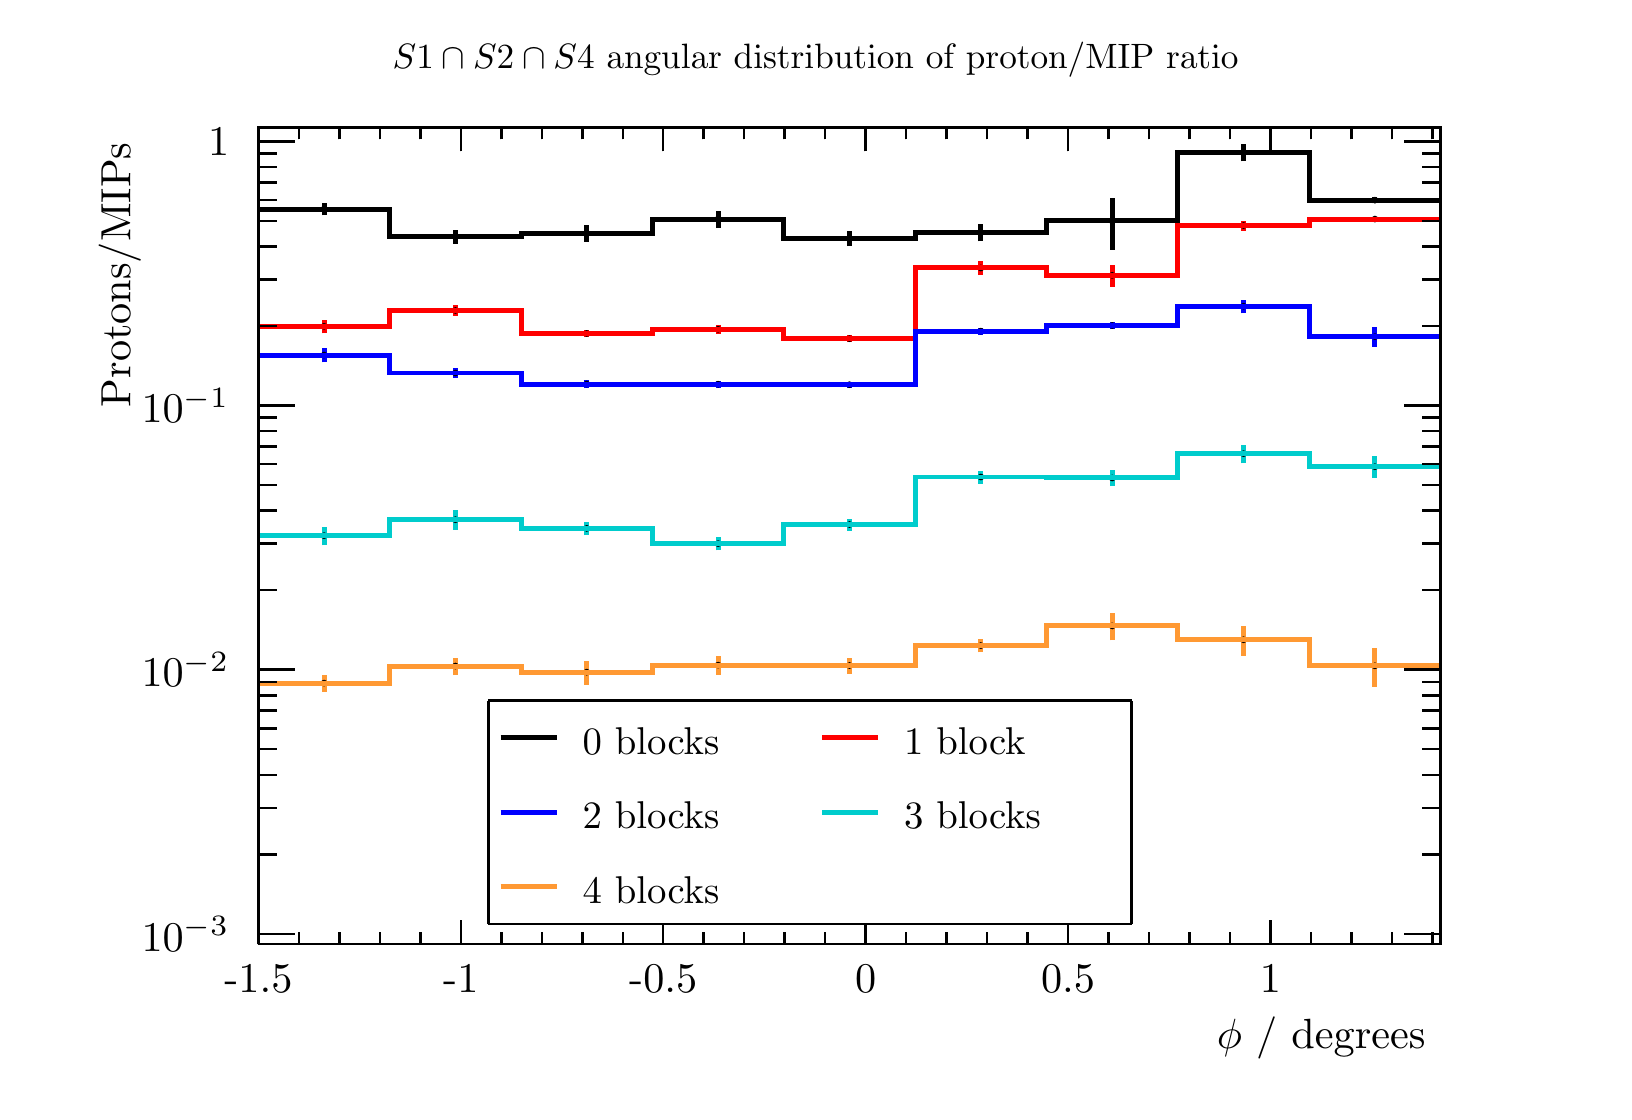
\begin{tikzpicture}
\pgfdeclareplotmark{cross} {
\pgfpathmoveto{\pgfpoint{-0.3\pgfplotmarksize}{\pgfplotmarksize}}
\pgfpathlineto{\pgfpoint{+0.3\pgfplotmarksize}{\pgfplotmarksize}}
\pgfpathlineto{\pgfpoint{+0.3\pgfplotmarksize}{0.3\pgfplotmarksize}}
\pgfpathlineto{\pgfpoint{+1\pgfplotmarksize}{0.3\pgfplotmarksize}}
\pgfpathlineto{\pgfpoint{+1\pgfplotmarksize}{-0.3\pgfplotmarksize}}
\pgfpathlineto{\pgfpoint{+0.3\pgfplotmarksize}{-0.3\pgfplotmarksize}}
\pgfpathlineto{\pgfpoint{+0.3\pgfplotmarksize}{-1.\pgfplotmarksize}}
\pgfpathlineto{\pgfpoint{-0.3\pgfplotmarksize}{-1.\pgfplotmarksize}}
\pgfpathlineto{\pgfpoint{-0.3\pgfplotmarksize}{-0.3\pgfplotmarksize}}
\pgfpathlineto{\pgfpoint{-1.\pgfplotmarksize}{-0.3\pgfplotmarksize}}
\pgfpathlineto{\pgfpoint{-1.\pgfplotmarksize}{0.3\pgfplotmarksize}}
\pgfpathlineto{\pgfpoint{-0.3\pgfplotmarksize}{0.3\pgfplotmarksize}}
\pgfpathclose
\pgfusepathqstroke
}
\pgfdeclareplotmark{cross*} {
\pgfpathmoveto{\pgfpoint{-0.3\pgfplotmarksize}{\pgfplotmarksize}}
\pgfpathlineto{\pgfpoint{+0.3\pgfplotmarksize}{\pgfplotmarksize}}
\pgfpathlineto{\pgfpoint{+0.3\pgfplotmarksize}{0.3\pgfplotmarksize}}
\pgfpathlineto{\pgfpoint{+1\pgfplotmarksize}{0.3\pgfplotmarksize}}
\pgfpathlineto{\pgfpoint{+1\pgfplotmarksize}{-0.3\pgfplotmarksize}}
\pgfpathlineto{\pgfpoint{+0.3\pgfplotmarksize}{-0.3\pgfplotmarksize}}
\pgfpathlineto{\pgfpoint{+0.3\pgfplotmarksize}{-1.\pgfplotmarksize}}
\pgfpathlineto{\pgfpoint{-0.3\pgfplotmarksize}{-1.\pgfplotmarksize}}
\pgfpathlineto{\pgfpoint{-0.3\pgfplotmarksize}{-0.3\pgfplotmarksize}}
\pgfpathlineto{\pgfpoint{-1.\pgfplotmarksize}{-0.3\pgfplotmarksize}}
\pgfpathlineto{\pgfpoint{-1.\pgfplotmarksize}{0.3\pgfplotmarksize}}
\pgfpathlineto{\pgfpoint{-0.3\pgfplotmarksize}{0.3\pgfplotmarksize}}
\pgfpathclose
\pgfusepathqfillstroke
}
\pgfdeclareplotmark{newstar} {
\pgfpathmoveto{\pgfqpoint{0pt}{\pgfplotmarksize}}
\pgfpathlineto{\pgfqpointpolar{44}{0.5\pgfplotmarksize}}
\pgfpathlineto{\pgfqpointpolar{18}{\pgfplotmarksize}}
\pgfpathlineto{\pgfqpointpolar{-20}{0.5\pgfplotmarksize}}
\pgfpathlineto{\pgfqpointpolar{-54}{\pgfplotmarksize}}
\pgfpathlineto{\pgfqpointpolar{-90}{0.5\pgfplotmarksize}}
\pgfpathlineto{\pgfqpointpolar{234}{\pgfplotmarksize}}
\pgfpathlineto{\pgfqpointpolar{198}{0.5\pgfplotmarksize}}
\pgfpathlineto{\pgfqpointpolar{162}{\pgfplotmarksize}}
\pgfpathlineto{\pgfqpointpolar{134}{0.5\pgfplotmarksize}}
\pgfpathclose
\pgfusepathqstroke
}
\pgfdeclareplotmark{newstar*} {
\pgfpathmoveto{\pgfqpoint{0pt}{\pgfplotmarksize}}
\pgfpathlineto{\pgfqpointpolar{44}{0.5\pgfplotmarksize}}
\pgfpathlineto{\pgfqpointpolar{18}{\pgfplotmarksize}}
\pgfpathlineto{\pgfqpointpolar{-20}{0.5\pgfplotmarksize}}
\pgfpathlineto{\pgfqpointpolar{-54}{\pgfplotmarksize}}
\pgfpathlineto{\pgfqpointpolar{-90}{0.5\pgfplotmarksize}}
\pgfpathlineto{\pgfqpointpolar{234}{\pgfplotmarksize}}
\pgfpathlineto{\pgfqpointpolar{198}{0.5\pgfplotmarksize}}
\pgfpathlineto{\pgfqpointpolar{162}{\pgfplotmarksize}}
\pgfpathlineto{\pgfqpointpolar{134}{0.5\pgfplotmarksize}}
\pgfpathclose
\pgfusepathqfillstroke
}
\definecolor{c}{rgb}{1,1,1};
\draw [color=c, fill=c] (0,0) rectangle (20,13.4957);
\draw [color=c, fill=c] (2.92264,1.86246) rectangle (17.937,12.235);
\definecolor{c}{rgb}{0,0,0};
\draw [c,line width=0.9] (2.92264,1.86246) -- (2.92264,12.235) -- (17.937,12.235) -- (17.937,1.86246) -- (2.92264,1.86246);
\definecolor{c}{rgb}{1,1,1};
\draw [color=c, fill=c] (2.92264,1.86246) rectangle (17.937,12.235);
\definecolor{c}{rgb}{0,0,0};
\draw [c,line width=0.9] (2.92264,1.86246) -- (2.92264,12.235) -- (17.937,12.235) -- (17.937,1.86246) -- (2.92264,1.86246);
\draw [c,line width=0.9] (2.92264,1.86246) -- (4.59089,1.86246) -- (4.59089,1.86246) -- (6.25915,1.86246) -- (6.25915,1.86246) -- (7.92741,1.86246) -- (7.92741,1.86246) -- (9.59567,1.86246) -- (9.59567,1.86246) -- (11.2639,1.86246) --
 (11.2639,1.86246) -- (12.9322,1.86246) -- (12.9322,1.86246) -- (14.6004,1.86246) -- (14.6004,1.86246) -- (16.2687,1.86246) -- (16.2687,1.86246) -- (17.937,1.86246);
\draw [c,line width=0.9] (2.92264,1.86246) -- (17.937,1.86246);
\draw [c,line width=0.9] (2.92264,2.16641) -- (2.92264,1.86246);
\draw [c,line width=0.9] (3.43683,2.01444) -- (3.43683,1.86246);
\draw [c,line width=0.9] (3.95101,2.01444) -- (3.95101,1.86246);
\draw [c,line width=0.9] (4.4652,2.01444) -- (4.4652,1.86246);
\draw [c,line width=0.9] (4.97939,2.01444) -- (4.97939,1.86246);
\draw [c,line width=0.9] (5.49358,2.16641) -- (5.49358,1.86246);
\draw [c,line width=0.9] (6.00777,2.01444) -- (6.00777,1.86246);
\draw [c,line width=0.9] (6.52196,2.01444) -- (6.52196,1.86246);
\draw [c,line width=0.9] (7.03615,2.01444) -- (7.03615,1.86246);
\draw [c,line width=0.9] (7.55034,2.01444) -- (7.55034,1.86246);
\draw [c,line width=0.9] (8.06453,2.16641) -- (8.06453,1.86246);
\draw [c,line width=0.9] (8.57872,2.01444) -- (8.57872,1.86246);
\draw [c,line width=0.9] (9.09291,2.01444) -- (9.09291,1.86246);
\draw [c,line width=0.9] (9.6071,2.01444) -- (9.6071,1.86246);
\draw [c,line width=0.9] (10.1213,2.01444) -- (10.1213,1.86246);
\draw [c,line width=0.9] (10.6355,2.16641) -- (10.6355,1.86246);
\draw [c,line width=0.9] (11.1497,2.01444) -- (11.1497,1.86246);
\draw [c,line width=0.9] (11.6639,2.01444) -- (11.6639,1.86246);
\draw [c,line width=0.9] (12.178,2.01444) -- (12.178,1.86246);
\draw [c,line width=0.9] (12.6922,2.01444) -- (12.6922,1.86246);
\draw [c,line width=0.9] (13.2064,2.16641) -- (13.2064,1.86246);
\draw [c,line width=0.9] (13.7206,2.01444) -- (13.7206,1.86246);
\draw [c,line width=0.9] (14.2348,2.01444) -- (14.2348,1.86246);
\draw [c,line width=0.9] (14.749,2.01444) -- (14.749,1.86246);
\draw [c,line width=0.9] (15.2632,2.01444) -- (15.2632,1.86246);
\draw [c,line width=0.9] (15.7774,2.16641) -- (15.7774,1.86246);
\draw [c,line width=0.9] (15.7774,2.16641) -- (15.7774,1.86246);
\draw [c,line width=0.9] (16.2916,2.01444) -- (16.2916,1.86246);
\draw [c,line width=0.9] (16.8057,2.01444) -- (16.8057,1.86246);
\draw [c,line width=0.9] (17.3199,2.01444) -- (17.3199,1.86246);
\draw [c,line width=0.9] (17.8341,2.01444) -- (17.8341,1.86246);
\draw [anchor=base] (2.92264,1.25516) node[scale=1.52731, color=c, rotate=0]{-1.5};
\draw [anchor=base] (5.49358,1.25516) node[scale=1.52731, color=c, rotate=0]{-1};
\draw [anchor=base] (8.06453,1.25516) node[scale=1.52731, color=c, rotate=0]{-0.5};
\draw [anchor=base] (10.6355,1.25516) node[scale=1.52731, color=c, rotate=0]{0};
\draw [anchor=base] (13.2064,1.25516) node[scale=1.52731, color=c, rotate=0]{0.5};
\draw [anchor=base] (15.7774,1.25516) node[scale=1.52731, color=c, rotate=0]{1};
\draw [anchor= east] (17.937,0.674842) node[scale=1.52731, color=c, rotate=0]{$\phi$ / degrees};
\draw [c,line width=0.9] (2.92264,12.235) -- (17.937,12.235);
\draw [c,line width=0.9] (2.92264,11.931) -- (2.92264,12.235);
\draw [c,line width=0.9] (3.43683,12.083) -- (3.43683,12.235);
\draw [c,line width=0.9] (3.95101,12.083) -- (3.95101,12.235);
\draw [c,line width=0.9] (4.4652,12.083) -- (4.4652,12.235);
\draw [c,line width=0.9] (4.97939,12.083) -- (4.97939,12.235);
\draw [c,line width=0.9] (5.49358,11.931) -- (5.49358,12.235);
\draw [c,line width=0.9] (6.00777,12.083) -- (6.00777,12.235);
\draw [c,line width=0.9] (6.52196,12.083) -- (6.52196,12.235);
\draw [c,line width=0.9] (7.03615,12.083) -- (7.03615,12.235);
\draw [c,line width=0.9] (7.55034,12.083) -- (7.55034,12.235);
\draw [c,line width=0.9] (8.06453,11.931) -- (8.06453,12.235);
\draw [c,line width=0.9] (8.57872,12.083) -- (8.57872,12.235);
\draw [c,line width=0.9] (9.09291,12.083) -- (9.09291,12.235);
\draw [c,line width=0.9] (9.6071,12.083) -- (9.6071,12.235);
\draw [c,line width=0.9] (10.1213,12.083) -- (10.1213,12.235);
\draw [c,line width=0.9] (10.6355,11.931) -- (10.6355,12.235);
\draw [c,line width=0.9] (11.1497,12.083) -- (11.1497,12.235);
\draw [c,line width=0.9] (11.6639,12.083) -- (11.6639,12.235);
\draw [c,line width=0.9] (12.178,12.083) -- (12.178,12.235);
\draw [c,line width=0.9] (12.6922,12.083) -- (12.6922,12.235);
\draw [c,line width=0.9] (13.2064,11.931) -- (13.2064,12.235);
\draw [c,line width=0.9] (13.7206,12.083) -- (13.7206,12.235);
\draw [c,line width=0.9] (14.2348,12.083) -- (14.2348,12.235);
\draw [c,line width=0.9] (14.749,12.083) -- (14.749,12.235);
\draw [c,line width=0.9] (15.2632,12.083) -- (15.2632,12.235);
\draw [c,line width=0.9] (15.7774,11.931) -- (15.7774,12.235);
\draw [c,line width=0.9] (15.7774,11.931) -- (15.7774,12.235);
\draw [c,line width=0.9] (16.2916,12.083) -- (16.2916,12.235);
\draw [c,line width=0.9] (16.8057,12.083) -- (16.8057,12.235);
\draw [c,line width=0.9] (17.3199,12.083) -- (17.3199,12.235);
\draw [c,line width=0.9] (17.8341,12.083) -- (17.8341,12.235);
\draw [c,line width=0.9] (2.92264,1.86246) -- (2.92264,12.235);
\draw [c,line width=0.9] (3.38378,1.99437) -- (2.92264,1.99437);
\draw [anchor= east] (2.74264,1.99437) node[scale=1.52731, color=c, rotate=0]{$10^{-3}$};
\draw [c,line width=0.9] (3.15321,3.00417) -- (2.92264,3.00417);
\draw [c,line width=0.9] (3.15321,3.59487) -- (2.92264,3.59487);
\draw [c,line width=0.9] (3.15321,4.01397) -- (2.92264,4.01397);
\draw [c,line width=0.9] (3.15321,4.33905) -- (2.92264,4.33905);
\draw [c,line width=0.9] (3.15321,4.60467) -- (2.92264,4.60467);
\draw [c,line width=0.9] (3.15321,4.82924) -- (2.92264,4.82924);
\draw [c,line width=0.9] (3.15321,5.02377) -- (2.92264,5.02377);
\draw [c,line width=0.9] (3.15321,5.19536) -- (2.92264,5.19536);
\draw [c,line width=0.9] (3.38378,5.34885) -- (2.92264,5.34885);
\draw [anchor= east] (2.74264,5.34885) node[scale=1.52731, color=c, rotate=0]{$10^{-2}$};
\draw [c,line width=0.9] (3.15321,6.35865) -- (2.92264,6.35865);
\draw [c,line width=0.9] (3.15321,6.94935) -- (2.92264,6.94935);
\draw [c,line width=0.9] (3.15321,7.36845) -- (2.92264,7.36845);
\draw [c,line width=0.9] (3.15321,7.69353) -- (2.92264,7.69353);
\draw [c,line width=0.9] (3.15321,7.95915) -- (2.92264,7.95915);
\draw [c,line width=0.9] (3.15321,8.18372) -- (2.92264,8.18372);
\draw [c,line width=0.9] (3.15321,8.37825) -- (2.92264,8.37825);
\draw [c,line width=0.9] (3.15321,8.54984) -- (2.92264,8.54984);
\draw [c,line width=0.9] (3.38378,8.70333) -- (2.92264,8.70333);
\draw [anchor= east] (2.74264,8.70333) node[scale=1.52731, color=c, rotate=0]{$10^{-1}$};
\draw [c,line width=0.9] (3.15321,9.71313) -- (2.92264,9.71313);
\draw [c,line width=0.9] (3.15321,10.3038) -- (2.92264,10.3038);
\draw [c,line width=0.9] (3.15321,10.7229) -- (2.92264,10.7229);
\draw [c,line width=0.9] (3.15321,11.048) -- (2.92264,11.048);
\draw [c,line width=0.9] (3.15321,11.3136) -- (2.92264,11.3136);
\draw [c,line width=0.9] (3.15321,11.5382) -- (2.92264,11.5382);
\draw [c,line width=0.9] (3.15321,11.7327) -- (2.92264,11.7327);
\draw [c,line width=0.9] (3.15321,11.9043) -- (2.92264,11.9043);
\draw [c,line width=0.9] (3.38378,12.0578) -- (2.92264,12.0578);
\draw [anchor= east] (2.74264,12.0578) node[scale=1.52731, color=c, rotate=0]{1};
\draw [anchor= east] (1.16264,12.235) node[scale=1.52731, color=c, rotate=90]{ Protons/MIPs};
\draw [c,line width=0.9] (17.937,1.86246) -- (17.937,12.235);
\draw [c,line width=0.9] (17.4758,1.99437) -- (17.937,1.99437);
\draw [c,line width=0.9] (17.7064,3.00417) -- (17.937,3.00417);
\draw [c,line width=0.9] (17.7064,3.59487) -- (17.937,3.59487);
\draw [c,line width=0.9] (17.7064,4.01397) -- (17.937,4.01397);
\draw [c,line width=0.9] (17.7064,4.33905) -- (17.937,4.33905);
\draw [c,line width=0.9] (17.7064,4.60467) -- (17.937,4.60467);
\draw [c,line width=0.9] (17.7064,4.82924) -- (17.937,4.82924);
\draw [c,line width=0.9] (17.7064,5.02377) -- (17.937,5.02377);
\draw [c,line width=0.9] (17.7064,5.19536) -- (17.937,5.19536);
\draw [c,line width=0.9] (17.4758,5.34885) -- (17.937,5.34885);
\draw [c,line width=0.9] (17.7064,6.35865) -- (17.937,6.35865);
\draw [c,line width=0.9] (17.7064,6.94935) -- (17.937,6.94935);
\draw [c,line width=0.9] (17.7064,7.36845) -- (17.937,7.36845);
\draw [c,line width=0.9] (17.7064,7.69353) -- (17.937,7.69353);
\draw [c,line width=0.9] (17.7064,7.95915) -- (17.937,7.95915);
\draw [c,line width=0.9] (17.7064,8.18372) -- (17.937,8.18372);
\draw [c,line width=0.9] (17.7064,8.37825) -- (17.937,8.37825);
\draw [c,line width=0.9] (17.7064,8.54984) -- (17.937,8.54984);
\draw [c,line width=0.9] (17.4758,8.70333) -- (17.937,8.70333);
\draw [c,line width=0.9] (17.7064,9.71313) -- (17.937,9.71313);
\draw [c,line width=0.9] (17.7064,10.3038) -- (17.937,10.3038);
\draw [c,line width=0.9] (17.7064,10.7229) -- (17.937,10.7229);
\draw [c,line width=0.9] (17.7064,11.048) -- (17.937,11.048);
\draw [c,line width=0.9] (17.7064,11.3136) -- (17.937,11.3136);
\draw [c,line width=0.9] (17.7064,11.5382) -- (17.937,11.5382);
\draw [c,line width=0.9] (17.7064,11.7327) -- (17.937,11.7327);
\draw [c,line width=0.9] (17.7064,11.9043) -- (17.937,11.9043);
\draw [c,line width=0.9] (17.4758,12.0578) -- (17.937,12.0578);
\draw [c,line width=1.8] (3.75677,11.1186) -- (3.75677,11.1994);
\draw [c,line width=1.8] (3.75677,11.1994) -- (3.75677,11.2759);
\foreach \P in {(3.75677,11.1994)}{\draw[mark options={color=c,fill=c},mark size=2.402402pt,mark=*,mark size=1pt] plot coordinates {\P};}
\draw [c,line width=1.8] (5.42502,10.7582) -- (5.42502,10.8484);
\draw [c,line width=1.8] (5.42502,10.8484) -- (5.42502,10.9333);
\foreach \P in {(5.42502,10.8484)}{\draw[mark options={color=c,fill=c},mark size=2.402402pt,mark=*,mark size=1pt] plot coordinates {\P};}
\draw [c,line width=1.8] (7.09328,10.781) -- (7.09328,10.891);
\draw [c,line width=1.8] (7.09328,10.891) -- (7.09328,10.9934);
\foreach \P in {(7.09328,10.891)}{\draw[mark options={color=c,fill=c},mark size=2.402402pt,mark=*,mark size=1pt] plot coordinates {\P};}
\draw [c,line width=1.8] (8.76154,10.9584) -- (8.76154,11.0722);
\draw [c,line width=1.8] (8.76154,11.0722) -- (8.76154,11.1778);
\foreach \P in {(8.76154,11.0722)}{\draw[mark options={color=c,fill=c},mark size=2.402402pt,mark=*,mark size=1pt] plot coordinates {\P};}
\draw [c,line width=1.8] (10.4298,10.7292) -- (10.4298,10.829);
\draw [c,line width=1.8] (10.4298,10.829) -- (10.4298,10.9224);
\foreach \P in {(10.4298,10.829)}{\draw[mark options={color=c,fill=c},mark size=2.402402pt,mark=*,mark size=1pt] plot coordinates {\P};}
\draw [c,line width=1.8] (12.0981,10.7883) -- (12.0981,10.9003);
\draw [c,line width=1.8] (12.0981,10.9003) -- (12.0981,11.0043);
\foreach \P in {(12.0981,10.9003)}{\draw[mark options={color=c,fill=c},mark size=2.402402pt,mark=*,mark size=1pt] plot coordinates {\P};}
\draw [c,line width=1.8] (13.7663,10.6792) -- (13.7663,11.0491);
\draw [c,line width=1.8] (13.7663,11.0491) -- (13.7663,11.3439);
\foreach \P in {(13.7663,11.0491)}{\draw[mark options={color=c,fill=c},mark size=2.402402pt,mark=*,mark size=1pt] plot coordinates {\P};}
\draw [c,line width=1.8] (15.4346,11.805) -- (15.4346,11.9179);
\draw [c,line width=1.8] (15.4346,11.9179) -- (15.4346,12.0227);
\foreach \P in {(15.4346,11.9179)}{\draw[mark options={color=c,fill=c},mark size=2.402402pt,mark=*,mark size=1pt] plot coordinates {\P};}
\draw [c,line width=1.8] (17.1028,11.2701) -- (17.1028,11.3119);
\draw [c,line width=1.8] (17.1028,11.3119) -- (17.1028,11.3525);
\foreach \P in {(17.1028,11.3119)}{\draw[mark options={color=c,fill=c},mark size=2.402402pt,mark=*,mark size=1pt] plot coordinates {\P};}
\draw [c,line width=1.8] (2.92264,11.1994) -- (4.59089,11.1994) -- (4.59089,10.8484) -- (6.25915,10.8484) -- (6.25915,10.891) -- (7.92741,10.891) -- (7.92741,11.0722) -- (9.59567,11.0722) -- (9.59567,10.829) -- (11.2639,10.829) -- (11.2639,10.9003)
 -- (12.9322,10.9003) -- (12.9322,11.0491) -- (14.6004,11.0491) -- (14.6004,11.9179) -- (16.2687,11.9179) -- (16.2687,11.3119) -- (17.937,11.3119);
\definecolor{c}{rgb}{1,0,0};
\draw [c,line width=1.8] (3.75677,9.62119) -- (3.75677,9.70959);
\draw [c,line width=1.8] (3.75677,9.70959) -- (3.75677,9.79292);
\definecolor{c}{rgb}{0,0,0};
\foreach \P in {(3.75677,9.70959)}{\draw[mark options={color=c,fill=c},mark size=2.402402pt,mark=*,mark size=1pt] plot coordinates {\P};}
\definecolor{c}{rgb}{1,0,0};
\draw [c,line width=1.8] (5.42502,9.84304) -- (5.42502,9.91121);
\draw [c,line width=1.8] (5.42502,9.91121) -- (5.42502,9.97633);
\definecolor{c}{rgb}{0,0,0};
\foreach \P in {(5.42502,9.91121)}{\draw[mark options={color=c,fill=c},mark size=2.402402pt,mark=*,mark size=1pt] plot coordinates {\P};}
\definecolor{c}{rgb}{1,0,0};
\draw [c,line width=1.8] (7.09328,9.57184) -- (7.09328,9.61898);
\draw [c,line width=1.8] (7.09328,9.61898) -- (7.09328,9.66464);
\definecolor{c}{rgb}{0,0,0};
\foreach \P in {(7.09328,9.61898)}{\draw[mark options={color=c,fill=c},mark size=2.402402pt,mark=*,mark size=1pt] plot coordinates {\P};}
\definecolor{c}{rgb}{1,0,0};
\draw [c,line width=1.8] (8.76154,9.61469) -- (8.76154,9.67266);
\draw [c,line width=1.8] (8.76154,9.67266) -- (8.76154,9.72841);
\definecolor{c}{rgb}{0,0,0};
\foreach \P in {(8.76154,9.67266)}{\draw[mark options={color=c,fill=c},mark size=2.402402pt,mark=*,mark size=1pt] plot coordinates {\P};}
\definecolor{c}{rgb}{1,0,0};
\draw [c,line width=1.8] (10.4298,9.51052) -- (10.4298,9.55301);
\draw [c,line width=1.8] (10.4298,9.55301) -- (10.4298,9.59431);
\definecolor{c}{rgb}{0,0,0};
\foreach \P in {(10.4298,9.55301)}{\draw[mark options={color=c,fill=c},mark size=2.402402pt,mark=*,mark size=1pt] plot coordinates {\P};}
\definecolor{c}{rgb}{1,0,0};
\draw [c,line width=1.8] (12.0981,10.3603) -- (12.0981,10.4511);
\draw [c,line width=1.8] (12.0981,10.4511) -- (12.0981,10.5365);
\definecolor{c}{rgb}{0,0,0};
\foreach \P in {(12.0981,10.4511)}{\draw[mark options={color=c,fill=c},mark size=2.402402pt,mark=*,mark size=1pt] plot coordinates {\P};}
\definecolor{c}{rgb}{1,0,0};
\draw [c,line width=1.8] (13.7663,10.2133) -- (13.7663,10.3573);
\draw [c,line width=1.8] (13.7663,10.3573) -- (13.7663,10.4882);
\definecolor{c}{rgb}{0,0,0};
\foreach \P in {(13.7663,10.3573)}{\draw[mark options={color=c,fill=c},mark size=2.402402pt,mark=*,mark size=1pt] plot coordinates {\P};}
\definecolor{c}{rgb}{1,0,0};
\draw [c,line width=1.8] (15.4346,10.9232) -- (15.4346,10.9897);
\draw [c,line width=1.8] (15.4346,10.9897) -- (15.4346,11.0534);
\definecolor{c}{rgb}{0,0,0};
\foreach \P in {(15.4346,10.9897)}{\draw[mark options={color=c,fill=c},mark size=2.402402pt,mark=*,mark size=1pt] plot coordinates {\P};}
\definecolor{c}{rgb}{1,0,0};
\draw [c,line width=1.8] (17.1028,11.0499) -- (17.1028,11.0718);
\draw [c,line width=1.8] (17.1028,11.0718) -- (17.1028,11.0934);
\definecolor{c}{rgb}{0,0,0};
\foreach \P in {(17.1028,11.0718)}{\draw[mark options={color=c,fill=c},mark size=2.402402pt,mark=*,mark size=1pt] plot coordinates {\P};}
\definecolor{c}{rgb}{1,0,0};
\draw [c,line width=1.8] (2.92264,9.70959) -- (4.59089,9.70959) -- (4.59089,9.91121) -- (6.25915,9.91121) -- (6.25915,9.61898) -- (7.92741,9.61898) -- (7.92741,9.67266) -- (9.59567,9.67266) -- (9.59567,9.55301) -- (11.2639,9.55301) --
 (11.2639,10.4511) -- (12.9322,10.4511) -- (12.9322,10.3573) -- (14.6004,10.3573) -- (14.6004,10.9897) -- (16.2687,10.9897) -- (16.2687,11.0718) -- (17.937,11.0718);
\definecolor{c}{rgb}{0,0,1};
\draw [c,line width=1.8] (3.75677,9.25151) -- (3.75677,9.34466);
\draw [c,line width=1.8] (3.75677,9.34466) -- (3.75677,9.43221);
\definecolor{c}{rgb}{0,0,0};
\foreach \P in {(3.75677,9.34466)}{\draw[mark options={color=c,fill=c},mark size=2.402402pt,mark=*,mark size=1pt] plot coordinates {\P};}
\definecolor{c}{rgb}{0,0,1};
\draw [c,line width=1.8] (5.42502,9.0576) -- (5.42502,9.11703);
\draw [c,line width=1.8] (5.42502,9.11703) -- (5.42502,9.17413);
\definecolor{c}{rgb}{0,0,0};
\foreach \P in {(5.42502,9.11703)}{\draw[mark options={color=c,fill=c},mark size=2.402402pt,mark=*,mark size=1pt] plot coordinates {\P};}
\definecolor{c}{rgb}{0,0,1};
\draw [c,line width=1.8] (7.09328,8.92432) -- (7.09328,8.97659);
\draw [c,line width=1.8] (7.09328,8.97659) -- (7.09328,9.02705);
\definecolor{c}{rgb}{0,0,0};
\foreach \P in {(7.09328,8.97659)}{\draw[mark options={color=c,fill=c},mark size=2.402402pt,mark=*,mark size=1pt] plot coordinates {\P};}
\definecolor{c}{rgb}{0,0,1};
\draw [c,line width=1.8] (8.76154,8.93085) -- (8.76154,8.9748);
\draw [c,line width=1.8] (8.76154,8.9748) -- (8.76154,9.01746);
\definecolor{c}{rgb}{0,0,0};
\foreach \P in {(8.76154,8.9748)}{\draw[mark options={color=c,fill=c},mark size=2.402402pt,mark=*,mark size=1pt] plot coordinates {\P};}
\definecolor{c}{rgb}{0,0,1};
\draw [c,line width=1.8] (10.4298,8.9314) -- (10.4298,8.96888);
\draw [c,line width=1.8] (10.4298,8.96888) -- (10.4298,9.00543);
\definecolor{c}{rgb}{0,0,0};
\foreach \P in {(10.4298,8.96888)}{\draw[mark options={color=c,fill=c},mark size=2.402402pt,mark=*,mark size=1pt] plot coordinates {\P};}
\definecolor{c}{rgb}{0,0,1};
\draw [c,line width=1.8] (12.0981,9.60358) -- (12.0981,9.64886);
\draw [c,line width=1.8] (12.0981,9.64886) -- (12.0981,9.69278);
\definecolor{c}{rgb}{0,0,0};
\foreach \P in {(12.0981,9.64886)}{\draw[mark options={color=c,fill=c},mark size=2.402402pt,mark=*,mark size=1pt] plot coordinates {\P};}
\definecolor{c}{rgb}{0,0,1};
\draw [c,line width=1.8] (13.7663,9.67288) -- (13.7663,9.71987);
\draw [c,line width=1.8] (13.7663,9.71987) -- (13.7663,9.76539);
\definecolor{c}{rgb}{0,0,0};
\foreach \P in {(13.7663,9.71987)}{\draw[mark options={color=c,fill=c},mark size=2.402402pt,mark=*,mark size=1pt] plot coordinates {\P};}
\definecolor{c}{rgb}{0,0,1};
\draw [c,line width=1.8] (15.4346,9.87473) -- (15.4346,9.9647);
\draw [c,line width=1.8] (15.4346,9.9647) -- (15.4346,10.0494);
\definecolor{c}{rgb}{0,0,0};
\foreach \P in {(15.4346,9.9647)}{\draw[mark options={color=c,fill=c},mark size=2.402402pt,mark=*,mark size=1pt] plot coordinates {\P};}
\definecolor{c}{rgb}{0,0,1};
\draw [c,line width=1.8] (17.1028,9.44819) -- (17.1028,9.57803);
\draw [c,line width=1.8] (17.1028,9.57803) -- (17.1028,9.69723);
\definecolor{c}{rgb}{0,0,0};
\foreach \P in {(17.1028,9.57803)}{\draw[mark options={color=c,fill=c},mark size=2.402402pt,mark=*,mark size=1pt] plot coordinates {\P};}
\definecolor{c}{rgb}{0,0,1};
\draw [c,line width=1.8] (2.92264,9.34466) -- (4.59089,9.34466) -- (4.59089,9.11703) -- (6.25915,9.11703) -- (6.25915,8.97659) -- (7.92741,8.97659) -- (7.92741,8.9748) -- (9.59567,8.9748) -- (9.59567,8.96888) -- (11.2639,8.96888) -- (11.2639,9.64886)
 -- (12.9322,9.64886) -- (12.9322,9.71987) -- (14.6004,9.71987) -- (14.6004,9.9647) -- (16.2687,9.9647) -- (16.2687,9.57803) -- (17.937,9.57803);
\definecolor{c}{rgb}{0,0.8,0.8};
\draw [c,line width=1.8] (3.75677,6.92902) -- (3.75677,7.05137);
\draw [c,line width=1.8] (3.75677,7.05137) -- (3.75677,7.16424);
\definecolor{c}{rgb}{0,0,0};
\foreach \P in {(3.75677,7.05137)}{\draw[mark options={color=c,fill=c},mark size=2.402402pt,mark=*,mark size=1pt] plot coordinates {\P};}
\definecolor{c}{rgb}{0,0.8,0.8};
\draw [c,line width=1.8] (5.42502,7.12655) -- (5.42502,7.25399);
\draw [c,line width=1.8] (5.42502,7.25399) -- (5.42502,7.37117);
\definecolor{c}{rgb}{0,0,0};
\foreach \P in {(5.42502,7.25399)}{\draw[mark options={color=c,fill=c},mark size=2.402402pt,mark=*,mark size=1pt] plot coordinates {\P};}
\definecolor{c}{rgb}{0,0.8,0.8};
\draw [c,line width=1.8] (7.09328,7.0589) -- (7.09328,7.1434);
\draw [c,line width=1.8] (7.09328,7.1434) -- (7.09328,7.22326);
\definecolor{c}{rgb}{0,0,0};
\foreach \P in {(7.09328,7.1434)}{\draw[mark options={color=c,fill=c},mark size=2.402402pt,mark=*,mark size=1pt] plot coordinates {\P};}
\definecolor{c}{rgb}{0,0.8,0.8};
\draw [c,line width=1.8] (8.76154,6.86461) -- (8.76154,6.95);
\draw [c,line width=1.8] (8.76154,6.95) -- (8.76154,7.03066);
\definecolor{c}{rgb}{0,0,0};
\foreach \P in {(8.76154,6.95)}{\draw[mark options={color=c,fill=c},mark size=2.402402pt,mark=*,mark size=1pt] plot coordinates {\P};}
\definecolor{c}{rgb}{0,0.8,0.8};
\draw [c,line width=1.8] (10.4298,7.1156) -- (10.4298,7.19278);
\draw [c,line width=1.8] (10.4298,7.19278) -- (10.4298,7.26608);
\definecolor{c}{rgb}{0,0,0};
\foreach \P in {(10.4298,7.19278)}{\draw[mark options={color=c,fill=c},mark size=2.402402pt,mark=*,mark size=1pt] plot coordinates {\P};}
\definecolor{c}{rgb}{0,0.8,0.8};
\draw [c,line width=1.8] (12.0981,7.71179) -- (12.0981,7.79608);
\draw [c,line width=1.8] (12.0981,7.79608) -- (12.0981,7.87577);
\definecolor{c}{rgb}{0,0,0};
\foreach \P in {(12.0981,7.79608)}{\draw[mark options={color=c,fill=c},mark size=2.402402pt,mark=*,mark size=1pt] plot coordinates {\P};}
\definecolor{c}{rgb}{0,0.8,0.8};
\draw [c,line width=1.8] (13.7663,7.67913) -- (13.7663,7.78379);
\draw [c,line width=1.8] (13.7663,7.78379) -- (13.7663,7.88143);
\definecolor{c}{rgb}{0,0,0};
\foreach \P in {(13.7663,7.78379)}{\draw[mark options={color=c,fill=c},mark size=2.402402pt,mark=*,mark size=1pt] plot coordinates {\P};}
\definecolor{c}{rgb}{0,0.8,0.8};
\draw [c,line width=1.8] (15.4346,7.97024) -- (15.4346,8.09262);
\draw [c,line width=1.8] (15.4346,8.09262) -- (15.4346,8.2055);
\definecolor{c}{rgb}{0,0,0};
\foreach \P in {(15.4346,8.09262)}{\draw[mark options={color=c,fill=c},mark size=2.402402pt,mark=*,mark size=1pt] plot coordinates {\P};}
\definecolor{c}{rgb}{0,0.8,0.8};
\draw [c,line width=1.8] (17.1028,7.78086) -- (17.1028,7.92626);
\draw [c,line width=1.8] (17.1028,7.92626) -- (17.1028,8.05845);
\definecolor{c}{rgb}{0,0,0};
\foreach \P in {(17.1028,7.92626)}{\draw[mark options={color=c,fill=c},mark size=2.402402pt,mark=*,mark size=1pt] plot coordinates {\P};}
\definecolor{c}{rgb}{0,0.8,0.8};
\draw [c,line width=1.8] (2.92264,7.05137) -- (4.59089,7.05137) -- (4.59089,7.25399) -- (6.25915,7.25399) -- (6.25915,7.1434) -- (7.92741,7.1434) -- (7.92741,6.95) -- (9.59567,6.95) -- (9.59567,7.19278) -- (11.2639,7.19278) -- (11.2639,7.79608) --
 (12.9322,7.79608) -- (12.9322,7.78379) -- (14.6004,7.78379) -- (14.6004,8.09262) -- (16.2687,8.09262) -- (16.2687,7.92626) -- (17.937,7.92626);
\definecolor{c}{rgb}{1,0.6,0.2};
\draw [c,line width=1.8] (3.75677,5.06881) -- (3.75677,5.1787);
\draw [c,line width=1.8] (3.75677,5.1787) -- (3.75677,5.28088);
\definecolor{c}{rgb}{0,0,0};
\foreach \P in {(3.75677,5.1787)}{\draw[mark options={color=c,fill=c},mark size=2.402402pt,mark=*,mark size=1pt] plot coordinates {\P};}
\definecolor{c}{rgb}{1,0.6,0.2};
\draw [c,line width=1.8] (5.42502,5.27915) -- (5.42502,5.3955);
\draw [c,line width=1.8] (5.42502,5.3955) -- (5.42502,5.50324);
\definecolor{c}{rgb}{0,0,0};
\foreach \P in {(5.42502,5.3955)}{\draw[mark options={color=c,fill=c},mark size=2.402402pt,mark=*,mark size=1pt] plot coordinates {\P};}
\definecolor{c}{rgb}{1,0.6,0.2};
\draw [c,line width=1.8] (7.09328,5.15626) -- (7.09328,5.31777);
\draw [c,line width=1.8] (7.09328,5.31777) -- (7.09328,5.46316);
\definecolor{c}{rgb}{0,0,0};
\foreach \P in {(7.09328,5.31777)}{\draw[mark options={color=c,fill=c},mark size=2.402402pt,mark=*,mark size=1pt] plot coordinates {\P};}
\definecolor{c}{rgb}{1,0.6,0.2};
\draw [c,line width=1.8] (8.76154,5.28414) -- (8.76154,5.40715);
\draw [c,line width=1.8] (8.76154,5.40715) -- (8.76154,5.52057);
\definecolor{c}{rgb}{0,0,0};
\foreach \P in {(8.76154,5.40715)}{\draw[mark options={color=c,fill=c},mark size=2.402402pt,mark=*,mark size=1pt] plot coordinates {\P};}
\definecolor{c}{rgb}{1,0.6,0.2};
\draw [c,line width=1.8] (10.4298,5.29775) -- (10.4298,5.4022);
\draw [c,line width=1.8] (10.4298,5.4022) -- (10.4298,5.49966);
\definecolor{c}{rgb}{0,0,0};
\foreach \P in {(10.4298,5.4022)}{\draw[mark options={color=c,fill=c},mark size=2.402402pt,mark=*,mark size=1pt] plot coordinates {\P};}
\definecolor{c}{rgb}{1,0.6,0.2};
\draw [c,line width=1.8] (12.0981,5.56964) -- (12.0981,5.65537);
\draw [c,line width=1.8] (12.0981,5.65537) -- (12.0981,5.73633);
\definecolor{c}{rgb}{0,0,0};
\foreach \P in {(12.0981,5.65537)}{\draw[mark options={color=c,fill=c},mark size=2.402402pt,mark=*,mark size=1pt] plot coordinates {\P};}
\definecolor{c}{rgb}{1,0.6,0.2};
\draw [c,line width=1.8] (13.7663,5.72272) -- (13.7663,5.90499);
\draw [c,line width=1.8] (13.7663,5.90499) -- (13.7663,6.06697);
\definecolor{c}{rgb}{0,0,0};
\foreach \P in {(13.7663,5.90499)}{\draw[mark options={color=c,fill=c},mark size=2.402402pt,mark=*,mark size=1pt] plot coordinates {\P};}
\definecolor{c}{rgb}{1,0.6,0.2};
\draw [c,line width=1.8] (15.4346,5.52494) -- (15.4346,5.72946);
\draw [c,line width=1.8] (15.4346,5.72946) -- (15.4346,5.90878);
\definecolor{c}{rgb}{0,0,0};
\foreach \P in {(15.4346,5.72946)}{\draw[mark options={color=c,fill=c},mark size=2.402402pt,mark=*,mark size=1pt] plot coordinates {\P};}
\definecolor{c}{rgb}{1,0.6,0.2};
\draw [c,line width=1.8] (17.1028,5.13287) -- (17.1028,5.39811);
\draw [c,line width=1.8] (17.1028,5.39811) -- (17.1028,5.62241);
\definecolor{c}{rgb}{0,0,0};
\foreach \P in {(17.1028,5.39811)}{\draw[mark options={color=c,fill=c},mark size=2.402402pt,mark=*,mark size=1pt] plot coordinates {\P};}
\definecolor{c}{rgb}{1,0.6,0.2};
\draw [c,line width=1.8] (2.92264,5.1787) -- (4.59089,5.1787) -- (4.59089,5.3955) -- (6.25915,5.3955) -- (6.25915,5.31777) -- (7.92741,5.31777) -- (7.92741,5.40715) -- (9.59567,5.40715) -- (9.59567,5.4022) -- (11.2639,5.4022) -- (11.2639,5.65537) --
 (12.9322,5.65537) -- (12.9322,5.90499) -- (14.6004,5.90499) -- (14.6004,5.72946) -- (16.2687,5.72946) -- (16.2687,5.39811) -- (17.937,5.39811);
\definecolor{c}{rgb}{0,0,0};
\draw [c,line width=0.9] (2.92264,1.86246) -- (17.937,1.86246);
\draw [c,line width=0.9] (2.92264,2.16641) -- (2.92264,1.86246);
\draw [c,line width=0.9] (3.43683,2.01444) -- (3.43683,1.86246);
\draw [c,line width=0.9] (3.95101,2.01444) -- (3.95101,1.86246);
\draw [c,line width=0.9] (4.4652,2.01444) -- (4.4652,1.86246);
\draw [c,line width=0.9] (4.97939,2.01444) -- (4.97939,1.86246);
\draw [c,line width=0.9] (5.49358,2.16641) -- (5.49358,1.86246);
\draw [c,line width=0.9] (6.00777,2.01444) -- (6.00777,1.86246);
\draw [c,line width=0.9] (6.52196,2.01444) -- (6.52196,1.86246);
\draw [c,line width=0.9] (7.03615,2.01444) -- (7.03615,1.86246);
\draw [c,line width=0.9] (7.55034,2.01444) -- (7.55034,1.86246);
\draw [c,line width=0.9] (8.06453,2.16641) -- (8.06453,1.86246);
\draw [c,line width=0.9] (8.57872,2.01444) -- (8.57872,1.86246);
\draw [c,line width=0.9] (9.09291,2.01444) -- (9.09291,1.86246);
\draw [c,line width=0.9] (9.6071,2.01444) -- (9.6071,1.86246);
\draw [c,line width=0.9] (10.1213,2.01444) -- (10.1213,1.86246);
\draw [c,line width=0.9] (10.6355,2.16641) -- (10.6355,1.86246);
\draw [c,line width=0.9] (11.1497,2.01444) -- (11.1497,1.86246);
\draw [c,line width=0.9] (11.6639,2.01444) -- (11.6639,1.86246);
\draw [c,line width=0.9] (12.178,2.01444) -- (12.178,1.86246);
\draw [c,line width=0.9] (12.6922,2.01444) -- (12.6922,1.86246);
\draw [c,line width=0.9] (13.2064,2.16641) -- (13.2064,1.86246);
\draw [c,line width=0.9] (13.7206,2.01444) -- (13.7206,1.86246);
\draw [c,line width=0.9] (14.2348,2.01444) -- (14.2348,1.86246);
\draw [c,line width=0.9] (14.749,2.01444) -- (14.749,1.86246);
\draw [c,line width=0.9] (15.2632,2.01444) -- (15.2632,1.86246);
\draw [c,line width=0.9] (15.7774,2.16641) -- (15.7774,1.86246);
\draw [c,line width=0.9] (15.7774,2.16641) -- (15.7774,1.86246);
\draw [c,line width=0.9] (16.2916,2.01444) -- (16.2916,1.86246);
\draw [c,line width=0.9] (16.8057,2.01444) -- (16.8057,1.86246);
\draw [c,line width=0.9] (17.3199,2.01444) -- (17.3199,1.86246);
\draw [c,line width=0.9] (17.8341,2.01444) -- (17.8341,1.86246);
\draw [c,line width=0.9] (2.92264,12.235) -- (17.937,12.235);
\draw [c,line width=0.9] (2.92264,11.931) -- (2.92264,12.235);
\draw [c,line width=0.9] (3.43683,12.083) -- (3.43683,12.235);
\draw [c,line width=0.9] (3.95101,12.083) -- (3.95101,12.235);
\draw [c,line width=0.9] (4.4652,12.083) -- (4.4652,12.235);
\draw [c,line width=0.9] (4.97939,12.083) -- (4.97939,12.235);
\draw [c,line width=0.9] (5.49358,11.931) -- (5.49358,12.235);
\draw [c,line width=0.9] (6.00777,12.083) -- (6.00777,12.235);
\draw [c,line width=0.9] (6.52196,12.083) -- (6.52196,12.235);
\draw [c,line width=0.9] (7.03615,12.083) -- (7.03615,12.235);
\draw [c,line width=0.9] (7.55034,12.083) -- (7.55034,12.235);
\draw [c,line width=0.9] (8.06453,11.931) -- (8.06453,12.235);
\draw [c,line width=0.9] (8.57872,12.083) -- (8.57872,12.235);
\draw [c,line width=0.9] (9.09291,12.083) -- (9.09291,12.235);
\draw [c,line width=0.9] (9.6071,12.083) -- (9.6071,12.235);
\draw [c,line width=0.9] (10.1213,12.083) -- (10.1213,12.235);
\draw [c,line width=0.9] (10.6355,11.931) -- (10.6355,12.235);
\draw [c,line width=0.9] (11.1497,12.083) -- (11.1497,12.235);
\draw [c,line width=0.9] (11.6639,12.083) -- (11.6639,12.235);
\draw [c,line width=0.9] (12.178,12.083) -- (12.178,12.235);
\draw [c,line width=0.9] (12.6922,12.083) -- (12.6922,12.235);
\draw [c,line width=0.9] (13.2064,11.931) -- (13.2064,12.235);
\draw [c,line width=0.9] (13.7206,12.083) -- (13.7206,12.235);
\draw [c,line width=0.9] (14.2348,12.083) -- (14.2348,12.235);
\draw [c,line width=0.9] (14.749,12.083) -- (14.749,12.235);
\draw [c,line width=0.9] (15.2632,12.083) -- (15.2632,12.235);
\draw [c,line width=0.9] (15.7774,11.931) -- (15.7774,12.235);
\draw [c,line width=0.9] (15.7774,11.931) -- (15.7774,12.235);
\draw [c,line width=0.9] (16.2916,12.083) -- (16.2916,12.235);
\draw [c,line width=0.9] (16.8057,12.083) -- (16.8057,12.235);
\draw [c,line width=0.9] (17.3199,12.083) -- (17.3199,12.235);
\draw [c,line width=0.9] (17.8341,12.083) -- (17.8341,12.235);
\draw [c,line width=0.9] (2.92264,1.86246) -- (2.92264,12.235);
\draw [c,line width=0.9] (3.38378,1.99437) -- (2.92264,1.99437);
\draw [c,line width=0.9] (3.15321,3.00417) -- (2.92264,3.00417);
\draw [c,line width=0.9] (3.15321,3.59487) -- (2.92264,3.59487);
\draw [c,line width=0.9] (3.15321,4.01397) -- (2.92264,4.01397);
\draw [c,line width=0.9] (3.15321,4.33905) -- (2.92264,4.33905);
\draw [c,line width=0.9] (3.15321,4.60467) -- (2.92264,4.60467);
\draw [c,line width=0.9] (3.15321,4.82924) -- (2.92264,4.82924);
\draw [c,line width=0.9] (3.15321,5.02377) -- (2.92264,5.02377);
\draw [c,line width=0.9] (3.15321,5.19536) -- (2.92264,5.19536);
\draw [c,line width=0.9] (3.38378,5.34885) -- (2.92264,5.34885);
\draw [c,line width=0.9] (3.15321,6.35865) -- (2.92264,6.35865);
\draw [c,line width=0.9] (3.15321,6.94935) -- (2.92264,6.94935);
\draw [c,line width=0.9] (3.15321,7.36845) -- (2.92264,7.36845);
\draw [c,line width=0.9] (3.15321,7.69353) -- (2.92264,7.69353);
\draw [c,line width=0.9] (3.15321,7.95915) -- (2.92264,7.95915);
\draw [c,line width=0.9] (3.15321,8.18372) -- (2.92264,8.18372);
\draw [c,line width=0.9] (3.15321,8.37825) -- (2.92264,8.37825);
\draw [c,line width=0.9] (3.15321,8.54984) -- (2.92264,8.54984);
\draw [c,line width=0.9] (3.38378,8.70333) -- (2.92264,8.70333);
\draw [c,line width=0.9] (3.15321,9.71313) -- (2.92264,9.71313);
\draw [c,line width=0.9] (3.15321,10.3038) -- (2.92264,10.3038);
\draw [c,line width=0.9] (3.15321,10.7229) -- (2.92264,10.7229);
\draw [c,line width=0.9] (3.15321,11.048) -- (2.92264,11.048);
\draw [c,line width=0.9] (3.15321,11.3136) -- (2.92264,11.3136);
\draw [c,line width=0.9] (3.15321,11.5382) -- (2.92264,11.5382);
\draw [c,line width=0.9] (3.15321,11.7327) -- (2.92264,11.7327);
\draw [c,line width=0.9] (3.15321,11.9043) -- (2.92264,11.9043);
\draw [c,line width=0.9] (3.38378,12.0578) -- (2.92264,12.0578);
\draw [c,line width=0.9] (17.937,1.86246) -- (17.937,12.235);
\draw [c,line width=0.9] (17.4758,1.99437) -- (17.937,1.99437);
\draw [c,line width=0.9] (17.7064,3.00417) -- (17.937,3.00417);
\draw [c,line width=0.9] (17.7064,3.59487) -- (17.937,3.59487);
\draw [c,line width=0.9] (17.7064,4.01397) -- (17.937,4.01397);
\draw [c,line width=0.9] (17.7064,4.33905) -- (17.937,4.33905);
\draw [c,line width=0.9] (17.7064,4.60467) -- (17.937,4.60467);
\draw [c,line width=0.9] (17.7064,4.82924) -- (17.937,4.82924);
\draw [c,line width=0.9] (17.7064,5.02377) -- (17.937,5.02377);
\draw [c,line width=0.9] (17.7064,5.19536) -- (17.937,5.19536);
\draw [c,line width=0.9] (17.4758,5.34885) -- (17.937,5.34885);
\draw [c,line width=0.9] (17.7064,6.35865) -- (17.937,6.35865);
\draw [c,line width=0.9] (17.7064,6.94935) -- (17.937,6.94935);
\draw [c,line width=0.9] (17.7064,7.36845) -- (17.937,7.36845);
\draw [c,line width=0.9] (17.7064,7.69353) -- (17.937,7.69353);
\draw [c,line width=0.9] (17.7064,7.95915) -- (17.937,7.95915);
\draw [c,line width=0.9] (17.7064,8.18372) -- (17.937,8.18372);
\draw [c,line width=0.9] (17.7064,8.37825) -- (17.937,8.37825);
\draw [c,line width=0.9] (17.7064,8.54984) -- (17.937,8.54984);
\draw [c,line width=0.9] (17.4758,8.70333) -- (17.937,8.70333);
\draw [c,line width=0.9] (17.7064,9.71313) -- (17.937,9.71313);
\draw [c,line width=0.9] (17.7064,10.3038) -- (17.937,10.3038);
\draw [c,line width=0.9] (17.7064,10.7229) -- (17.937,10.7229);
\draw [c,line width=0.9] (17.7064,11.048) -- (17.937,11.048);
\draw [c,line width=0.9] (17.7064,11.3136) -- (17.937,11.3136);
\draw [c,line width=0.9] (17.7064,11.5382) -- (17.937,11.5382);
\draw [c,line width=0.9] (17.7064,11.7327) -- (17.937,11.7327);
\draw [c,line width=0.9] (17.7064,11.9043) -- (17.937,11.9043);
\draw [c,line width=0.9] (17.4758,12.0578) -- (17.937,12.0578);
\definecolor{c}{rgb}{1,1,1};
\draw [color=c, fill=c] (2,12.7534) rectangle (18,13.4282);
\definecolor{c}{rgb}{0,0,0};
\draw (10,13.0908) node[scale=1.27276, color=c, rotate=0]{$S1 \cap S2 \cap S4$ angular distribution of proton/MIP ratio};
\definecolor{c}{rgb}{1,1,1};
\draw [color=c, fill=c] (5.84527,2.12034) rectangle (14.0115,4.95702);
\definecolor{c}{rgb}{0,0,0};
\draw [c,line width=0.9] (5.84527,2.12034) -- (14.0115,2.12034);
\draw [c,line width=0.9] (14.0115,2.12034) -- (14.0115,4.95702);
\draw [c,line width=0.9] (14.0115,4.95702) -- (5.84527,4.95702);
\draw [c,line width=0.9] (5.84527,4.95702) -- (5.84527,2.12034);
\draw [anchor=base west] (6.86605,4.27149) node[scale=1.40004, color=c, rotate=0]{0 blocks};
\draw [c,line width=1.8] (5.99839,4.48424) -- (6.71293,4.48424);
\draw [anchor=base west] (10.9491,4.27149) node[scale=1.40004, color=c, rotate=0]{1 block};
\definecolor{c}{rgb}{1,0,0};
\draw [c,line width=1.8] (10.0815,4.48424) -- (10.796,4.48424);
\definecolor{c}{rgb}{0,0,0};
\draw [anchor=base west] (6.86605,3.32593) node[scale=1.40004, color=c, rotate=0]{2 blocks};
\definecolor{c}{rgb}{0,0,1};
\draw [c,line width=1.8] (5.99839,3.53868) -- (6.71293,3.53868);
\definecolor{c}{rgb}{0,0,0};
\draw [anchor=base west] (10.9491,3.32593) node[scale=1.40004, color=c, rotate=0]{3 blocks};
\definecolor{c}{rgb}{0,0.8,0.8};
\draw [c,line width=1.8] (10.0815,3.53868) -- (10.796,3.53868);
\definecolor{c}{rgb}{0,0,0};
\draw [anchor=base west] (6.86605,2.38037) node[scale=1.40004, color=c, rotate=0]{4 blocks};
\definecolor{c}{rgb}{1,0.6,0.2};
\draw [c,line width=1.8] (5.99839,2.59312) -- (6.71293,2.59312);
\end{tikzpicture}
